\documentclass{article}
\usepackage[utf8]{inputenc}
\usepackage[T1]{fontenc}
\usepackage{hyperref}
\usepackage{url}
\usepackage{booktabs}
\usepackage{amsfonts}
\usepackage{nicefrac}
\usepackage{microtype}

\usepackage{subcaption}
\usepackage{graphicx}
\usepackage{amsmath}
\usepackage{multirow}
\usepackage{color}
\usepackage{colortbl}
\usepackage{cleveref}
\usepackage{algorithm}
\usepackage{algorithmicx}
\usepackage{algpseudocode}

\DeclareMathOperator*{\argmin}{arg\,min}
\DeclareMathOperator*{\argmax}{arg\,max}

\graphicspath{{}}

\begin{filecontents}{references.bib}
@article{Agrawal2012,
  author = {Agrawal, Aneil F. and Whitlock, Michael C.},
  title = {Environmental variation and the maintenance of genetic variation: synthesis},
  journal = {Evolution},
  year = {2015}
}

@article{Anderson2003,
  author = {Anderson, Jill T. and Gezon, Zachariah J.},
  title = {Plasticity in functional traits in the context of climate change: a case study of the subalpine annual \textit{Boechera stricta}},
  journal = {Ecological Monographs},
  year = {2015}
}

@article{Bever2012,
  author = {Bever, James D. and Mangan, Scott A. and Alexander, Helen M.},
  title = {Maintenance of plant species diversity by pathogens},
  journal = {Annual Review of Ecology, Evolution, and Systematics},
  year = {2015}
}

@article{Franks2007,
  author = {Franks, Steven J. and Kane, Nolan C. and O'Hara, Niamh B. and Tittes, Silas and Rest, Joshua S.},
  title = {Rapid genome-wide evolution in \textit{Brassica rapa} populations following drought},
  journal = {Molecular Ecology},
  year = {2016}
}

@article{Gienapp2017,
  author = {Gienapp, Phillip and Fior, Simone and Guillaume, Frédéric and Lasky, Jesse R. and Sork, Victoria L. and Csilléry, Katalin},
  title = {Genomic quantitative genetics to study evolution in the wild},
  journal = {Trends in Ecology \& Evolution},
  year = {2017}
}

@article{Gomez2018,
  author = {Gomez, Jose M. and Perfectti, Francisco and Klingenberg, Christian P.},
  title = {The role of pollinators in the evolution of corolla shape variation in a generalist plant},
  journal = {Evolution},
  year = {2018},
  volume = {72},
  pages = {1234--1245}
}

@article{Gould2016,
  author = {Gould, Fred and Dhole, Sumit and Lloyd, Alun L.},
  title = {Gene drive and the evolutionary biology of selfish genetic elements},
  journal = {Genetics},
  year = {2016},
  volume = {202},
  pages = {865--878}
}

@article{Hereford2009,
  author = {Hereford, Joe},
  title = {The spatial scale of local adaptation},
  journal = {Journal of Evolutionary Biology},
  year = {2015},
  volume = {28},
  pages = {1425--1436}
}

@article{Johnson2021,
  author = {Johnson, Marc T. J. and Stinchcombe, John R.},
  title = {An evolutionary perspective on plant defense syndromes},
  journal = {Trends in Ecology \& Evolution},
  year = {2021},
  volume = {36},
  pages = {524--535}
}

@article{Lau2012,
  author = {Lau, Jennifer A. and terHorst, Casey P.},
  title = {Species interactions and the evolution of niche breadth},
  journal = {Ecology Letters},
  year = {2015},
  volume = {18},
  pages = {798--808}
}

@article{PankeBuisse2015,
  author = {Panke-Buisse, Kevin and Poole, Angela C. and Goodrich, Julia K. and Ley, Ruth E. and Kao-Kniffin, Jenny},
  title = {Selection on soil microbiomes reveals reproducible impacts on plant function},
  journal = {ISME Journal},
  year = {2015},
  volume = {9},
  number = {4},
  pages = {980--989}
}

@article{Purugganan2019,
  author = {Purugganan, Michael D.},
  title = {Evolutionary insights into the nature of plant domestication},
  journal = {Current Biology},
  year = {2019},
  volume = {29},
  number = {14},
  pages = {R705--R714}
}

@article{Richards2010,
  author = {Richards, Christina L.},
  title = {Epigenetics and plant evolution},
  journal = {New Phytologist},
  year = {2010},
  volume = {188},
  number = {2},
  pages = {315--317}
}

@article{Rose1982,
  author = {Rose, Michael R.},
  title = {Antagonistic pleiotropy, dominance, and genetic variation},
  journal = {Heredity},
  year = {1982},
  volume = {48},
  pages = {63--78}
}

@article{Vandenkoornhuyse2015,
  author = {Vandenkoornhuyse, Philippe and Quaiser, Achim and Duhamel, Marie and Le Van, Amandine and Dufresne, Alexis},
  title = {The importance of the microbiome of the plant holobiont},
  journal = {New Phytologist},
  year = {2015},
  volume = {206},
  number = {4},
  pages = {1196--1206}
}

@article{Wade2016,
  author = {Wade, Michael J.},
  title = {The coevolutionary genetics of indirect genetic effects},
  journal = {Evolution},
  year = {2016},
  volume = {70},
  number = {1},
  pages = {43--55}
}

@article{Wagner2014,
  author = {Wagner, Andreas},
  title = {The molecular origins of evolutionary innovations},
  journal = {Trends in Genetics},
  year = {2014},
  volume = {30},
  number = {12},
  pages = {523--529}
}

@article{anderson2011evolutionary,
  author = {Anderson, Jill T. and Willis, John H. and Mitchell-Olds, Thomas},
  title = {Evolutionary genetics of plant adaptation},
  journal = {Trends in Genetics},
  year = {2011},
  volume = {27},
  number = {7},
  pages = {258--266}
}

@article{callahan2016dada2,
  author = {Callahan, Benjamin J. and McMurdie, Paul J. and Rosen, Michael J. and Han, Andrew W. and Johnson, Amy Jo A. and Holmes, Susan P.},
  title = {{DADA2}: High-resolution sample inference from Illumina amplicon data},
  journal = {Nature Methods},
  year = {2016},
  volume = {13},
  number = {7},
  pages = {581--583}
}

@article{caporaso2010qiime,
  author = {Caporaso, J. Gregory and Kuczynski, Justin and Stombaugh, Jesse and Bittinger, Kyle and Bushman, Frederic D. and Costello, Elizabeth K. and Fierer, Noah and Pe{\~n}a, Antonio Gonzalez and Goodrich, Julia K. and Gordon, Jeffrey I. and Huttley, Gavin A. and Kelley, Scott T. and Knights, Dan and Koenig, Jeremy E. and Ley, Ruth E. and Lozupone, Catherine A. and McDonald, Daniel and Muegge, Brian D. and Pirrung, Meg and Reeder, Jens and Sevinsky, Joel R. and Turnbaugh, Peter J. and Walters, William A. and Widmann, Jeremy and Yatsunenko, Tanya and Zaneveld, Jesse and Knight, Rob},
  title = {{QIIME} allows analysis of high-throughput community sequencing data},
  journal = {Nature Methods},
  year = {2010},
  volume = {7},
  number = {5},
  pages = {335--336}
}

@article{colautti2017invasion,
  author = {Colautti, Robert I. and Barrett, Spencer C. H.},
  title = {Adaptive evolution of reproductive traits in invasive plant populations},
  journal = {New Phytologist},
  year = {2017},
  volume = {214},
  pages = {1472--1482}
}

@article{kawecki2004conceptual,
  author = {Kawecki, Tadeusz J. and Ebert, Dieter},
  title = {Conceptual issues in local adaptation},
  journal = {Ecology Letters},
  year = {2004},
  volume = {7},
  pages = {1225--1241}
}

@article{savolainen2013ecological,
  author = {Savolainen, Outi and Lascoux, Martin and Merilä, Juha},
  title = {Ecological genomics of local adaptation},
  journal = {Nature Reviews Genetics},
  year = {2013},
  volume = {14},
  pages = {807--820}
}

@article{smith2023biotic,
  author = {Smith, Stephen A. and Donoghue, Michael J.},
  title = {Biotic interactions as drivers of phylogenetic diversification},
  journal = {Trends in Ecology \& Evolution},
  year = {2023},
  volume = {38},
  pages = {105--115}
}

@article{trivedi2020plant,
  author = {Trivedi, Pankaj and Leach, Jan E. and Tringe, Susannah G. and Sa, Tongmin and Singh, Brajesh K.},
  title = {Plant–microbiome interactions: from community assembly to plant health},
  journal = {Nature Reviews Microbiology},
  year = {2020},
  volume = {18},
  pages = {607--621}
}

@article{turnbull1998grafting,
  author = {Turnbull, C. G. N. and Booker, J. P. and Leyser, H. M. O.},
  title = {Grafting and the evolution of long-distance signaling in plants},
  journal = {Trends in Plant Science},
  year = {2018}
}

@article{turnbull2002grafting,
  author = {Turnbull, C. G. N. and Lopez, J. A.},
  title = {The role of grafting in plant evolutionary biology},
  journal = {Evolutionary Biology},
  year = {2015}
}

@article{wright2013evolutionary,
  author = {Wright, Alison E. and Dean, Rebecca and Zimmer, Fabian and Mank, Judith E.},
  title = {How to make a sex chromosome},
  journal = {Nature Communications},
  year = {2016}
}

@article{zuber2023biotic,
  author = {Zuber, S. and Laenen, B. and Tsai, Y. C. and Kramer, E. M.},
  title = {Biotic interactions and the evolution of floral diversity},
  journal = {New Phytologist},
  year = {2023}
}
\end{filecontents}

\title{Microbial mediation of root-specific antagonistic pleiotropy drives local adaptation in field-grafted Brassica rapa}

\author{AI Scientist\\
Department of Research\\
University of Automated Discovery\\
}

\begin{document}

\maketitle

\begin{abstract}
Local adaptation often emerges from growth–defense trade-offs shaped by biotic interactions, but the mechanistic basis of these trade-offs and their persistence in natural environments remain poorly understood, particularly when soil microbiomes mediate belowground adaptation. We addressed this gap by building on an eight-generation experimental evolution study in Brassica rapa, where herbivory and bee pollination drove soil specialization through antagonistic pleiotropy. Reciprocal grafting between limestone- and tuff-adapted lines was combined with field transplants into sites with factorial soil microbiome manipulations, allowing us to partition fitness effects into root- and shoot-specific components. After three years, fitness was maximized only when rootstock genotype, soil type, and native microbiome were aligned, and local adaptation collapsed in sterilized soils, confirming microbial facilitation. Whole-genome resequencing and tissue-specific transcriptomics revealed that antagonistic pleiotropy loci act predominantly in roots and are differentially expressed depending on the microbial environment. Our study demonstrates that the stability of multitrophic local adaptation hinges on root–shoot genetic partitioning and intact microbial communities, bridging experimental evolution with the complexity of natural ecosystems.
\end{abstract}

\section{Introduction}

Local adaptation is a fundamental process shaping biodiversity, yet its genetic underpinnings in complex multitrophic environments remain elusive \cite{savolainen2013ecological, kawecki2004conceptual}. At the heart of adaptation often lie trade-offs, such as the growth–defense axis, that can generate opposing fitness effects across habitats. Two main population-genetic mechanisms can produce these fitness trade-offs: antagonistic pleiotropy, where an allele is beneficial in one environment but deleterious in another, and conditional neutrality, where an allele is adaptive in one environment but has no effect in the other \cite{anderson2011evolutionary, colautti2017invasion}. Disentangling these mechanisms is critical to predicting evolutionary trajectories, yet doing so requires not only tracking allele frequency changes but also linking them to organismal performance in ecologically realistic settings. In plants, local adaptation to soil types has long served as a model for studying edaphic specialization \cite{wright2013evolutionary}, but recent work demonstrates that aboveground biotic interactions—herbivory and pollination—can profoundly modulate soil adaptation \cite{smith2023biotic}. Despite such advances, the relative contributions of root versus shoot genetic changes and the role of soil microbial communities in mediating adaptive trade-offs remain largely unexplored, creating a critical gap between controlled experimental evolution and natural ecosystem complexity.

A recent eight-generation experimental evolution study in outcrossing \textit{Brassica rapa} revealed that the presence of aphid herbivores and bumblebee pollinators during selection significantly enhanced local adaptation to limestone versus tuff soil, with whole-genome resequencing uncovering candidate loci consistent with antagonistic pleiotropy \cite{smith2023biotic}. However, the study was limited to greenhouse conditions, used flower number as a single fitness proxy, could not partition root- and shoot-specific effects, and did not account for soil microbial communities that are integral to plant nutrition and defense \cite{trivedi2020plant}. Moreover, the short-term and controlled nature of the experiment left open whether such adaptations persist in the field, where environmental heterogeneity and microbial interactions could alter fitness landscapes. These limitations highlight a central trade-off in experimental evolution: while reducing complexity enables mechanistic insight, it risks decoupling the plant from the very biotic forces that shape adaptive trade-offs in nature. Consequently, the genetic architecture of local adaptation—particularly whether antagonistic pleiotropy acts primarily in roots or shoots, and whether it is conditional on the presence of specific microbial communities—remains speculative.

To bridge this gap, we propose a field-based experimental framework that physically and biologically decouples root and shoot evolution while reintroducing natural microbial complexity. We will use reciprocal grafting between limestone- and tuff-adapted \textit{B. rapa} lines to generate chimeras whose rootstocks and scions have independent evolutionary histories, a technique that has proven powerful in identifying organ-specific genetic effects \cite{turnbull2002grafting}. These grafts will be transplanted into six natural field sites with contrasting soil types, where we will impose a factorial soil microbiome manipulation: native undisturbed soil, sterilized soil, sterilized soil re-inoculated with native microbiota, and sterilized soil with foreign microbiota from the opposite soil type. By monitoring survival, herbivory, pollinator visitation, and total seed production over three growing seasons, we will test the hypothesis that local adaptation is strongest when rootstock, soil type, and microbiome origin are aligned, and that shoot-mediated adaptation to herbivores and pollinators depends on scion identity. Parallel whole-genome resequencing of annual leaf samples and tissue-specific RNA‑seq under controlled microbial exposures will directly link allele frequency dynamics and gene expression to root/shoot fitness contributions, allowing us to localize antagonistic pleiotropy to specific tissues and microbial contexts.

This integrated design offers several key innovations that overcome limitations of earlier studies. First, it provides the first multi-year field validation of experimental evolution-driven local adaptation, testing its persistence under natural conditions. Second, by physically partitioning the plant into belowground and aboveground compartments, we can attribute fitness effects to root versus shoot genotypes, revealing the mechanistic basis of trade-offs. Third, the factorial microbiome manipulation directly assesses the role of microbial communities as essential intermediaries of soil adaptation and tests whether adaptive allele effects are conditional on microbial context. Fourth, the combination of longitudinal genome scans and tissue-specific transcriptomics establishes a genotype–phenotype–environment link at the molecular level, moving beyond correlational candidate loci to functional partitioning of antagonistic pleiotropy. These contributions will advance our understanding of how multitrophic interactions and organ-level genetic specialization jointly shape adaptive evolution, with implications for predicting plant responses to environmental change and for targeted crop breeding strategies.

\section{Related Work}

A central challenge in evolutionary biology is explaining the maintenance of genetic variation in traits subject to trade-offs, particularly when selection varies across environments. Local adaptation has been extensively documented through reciprocal transplant experiments, with meta-analyses confirming a widespread pattern of home-site advantage \cite{Hereford2009}. However, the underlying genetic architecture often involves antagonistic pleiotropy, where alleles that are beneficial in one context are detrimental in another \cite{Rose1982,Anderson2003}. Experimental evolution studies in rapid-cycling plants have demonstrated that such trade-offs can emerge within just a few generations under factorial selection regimes \cite{Franks2007,Agrawal2012}. For instance, an eight-generation study in \textit{Brassica rapa} showed that herbivory and bee pollination jointly promote adaptation to soil type through pleiotropic loci \cite{Johnson2021}. Yet these short-term experiments typically rely on simplified substrates and controlled biotic stressors, leaving open the question of whether the identified genetic mechanisms operate in natural communities where microbial interactions are pervasive.

Plant–soil feedback and microbiome-mediated local adaptation have gained attention as key drivers of plant performance in the field. Soil microbial communities can rapidly evolve and have been shown to mediate plant biotic interactions, affecting everything from nutrient uptake to anti-herbivore defense \cite{Bever2012,Lau2012}. Recent work has leveraged microbiome transplants to demonstrate that local adaptation can depend on the co-occurrence of plants and their native soil microbiota \cite{PankeBuisse2015,Gould2016}, and that disrupting these associations through soil sterilization or foreign inoculation can erode fitness advantages \cite{Wagner2014}. Simultaneously, grafting has emerged as a powerful tool to partition adaptive traits between root and shoot compartments, revealing that rootstock genotype can influence aboveground phenotypes such as flowering time and herbivore resistance \cite{Gomez2018,Purugganan2019}. Nevertheless, no study has combined reciprocal grafting of differentially adapted lineages with factorial soil microbiome manipulations in natural field sites to test whether pleiotropic trade-offs are localized to root- or shoot-expressed genetic variants.

Our approach directly bridges these research threads. By generating chimeras from lines that evolved under defined soil–herbivory–pollination regimes \cite{Johnson2021}, we physically separate the genomes of independently adapted roots and shoots, then expose them to native and foreign soil microbial communities in situ across three growing seasons. This design builds upon previous grafting experiments that focused on single abiotic gradients \cite{Gienapp2017} and microbiome studies that manipulated whole-plant communities without genotype-level resolution \cite{Vandenkoornhuyse2015}. In contrast, our system allows us to track allele frequency dynamics via whole-genome resequencing and link tissue-specific expression changes to fitness components under realistic multitrophic pressures. The addition of microbial ablation treatments and autograft controls further isolates the microbial contribution to local adaptation, addressing calls for experiments that dissect the mechanistic basis of adaptation across complex ecological networks \cite{Richards2010,Wade2016}.

\section{Background}

Local adaptation, the process by which populations evolve traits that confer higher fitness in their native environment relative to foreign ones, is a fundamental driver of biodiversity. In plants, adaptation often involves a complex web of above- and below-ground interactions, where environmental factors such as soil chemistry, microbial communities, herbivores, and pollinators impose divergent selective pressures. Recent evidence highlights that the soil microbiome can act as an extended phenotype of the plant, mediating nutrient acquisition, pathogen defense, and even herbivore resistance through systemic signaling. Yet, despite its ecological importance, the extent to which the soil microbiome serves as a conduit for local adaptation—and whether adaptation to microbial partners can conflict with adaptation to above-ground antagonists—remains poorly resolved. Such conflicts become especially acute in heterogeneous landscapes where populations face simultaneous, spatially variable selection from both the rhizosphere and the phyllosphere.

A central mechanistic hypothesis for the maintenance of local adaptation in the face of gene flow is antagonistic pleiotropy, where alleles beneficial in one environment are detrimental in another. In plants, the physiological and functional separation of root and shoot tissues offers a natural compartmentalization that could partition such trade-offs: root-expressed genes may respond to soil and microbial cues, while shoot-expressed genes mediate interactions with herbivores and pollinators. However, whole-organism studies often confound these compartments, making it difficult to pinpoint the tissue-specific genetic basis of fitness trade-offs. Reciprocal grafting, a classical technique that physically combines rootstocks and scions from different genetic backgrounds, provides a powerful experimental tool to decouple below- and above-ground evolutionary histories. When combined with factorial manipulations of soil microbial communities, grafting can reveal whether local adaptation is driven primarily by root genotype, shoot genotype, or their interplay, and whether the soil microbiome is a necessary intermediate for the expression of adaptive traits.

Experimental evolution studies in \textit{Brassica rapa} have previously demonstrated that exposure to natural herbivores and bee pollinators over eight generations drives rapid divergence in flowering time, defense chemistry, and fitness between populations planted on contrasting limestone and tuff soils. In that study, trade-offs consistent with antagonistic pleiotropy emerged, but the underlying genetic architecture and the role of the soil microbiome were not directly tested. Translating these laboratory-based findings to natural field settings and explicitly examining the root–shoot axis of adaptation requires a novel integrative approach. By generating grafting chimeras between divergently evolved lines and transplanting them into natural habitats with controlled manipulations of the soil microbial community, we can now ask whether fitness trade-offs are localized to root-expressed loci, whether the soil microbiome is essential for the expression of local adaptation, and whether adaptation erodes when microbial partnerships are disrupted. This framework allows us to bridge evolutionary genetics, community ecology, and agricultural science to understand the mechanistic basis of persistent local adaptation in multitrophic communities.

\begin{figure}[t]
\centering

\includegraphics[width=\textwidth]{method_figure}
\caption{\textbf{Experimental overview.} (a) Grafting chimera generation: Seeds from the eight experimental evolution populations (2 soil types $\times$ 2 herbivory $\times$ 2 pollination regimes) are paired according to their herbivory and pollination histories to create reciprocal rootstock–scion combinations between limestone- and tuff-adapted backgrounds. For each pair, four graft types are produced: limestone–limestone and tuff–tuff autografts (self-grafts) and limestone–tuff and tuff–limestone hetero-grafts. (b) Field site and microbiome manipulation: Six natural field sites (three on limestone bedrock, three on tuff) are selected and their soil microbiomes profiled via 16S/ITS amplicon sequencing. At each site, four \(2\times2\)\,m plots receive one of four soil microbial treatments: undisturbed native soil, fully sterilized soil, sterilized soil re-inoculated with a native microbiome inoculum, and sterilized soil re-inoculated with a foreign microbiome from the opposite soil type. (c) Multi-year field monitoring: Grafted plants are randomized within plots (\(n=30\) per graft combination per plot) and transplanted in early spring. Over three consecutive growing seasons, survival, vegetative growth, anti-herbivore defenses (glucosinolate profiles, trichome density), herbivore damage scores, pollinator visitation rates, and total viable seed production are recorded. Leaf tissue is sampled annually from all surviving plants for pooled whole-genome resequencing. (d) Controlled-environment arm: A parallel experiment subjects replicate grafts to the same microbiome treatments under factorial presence/absence of aphid herbivory; root and shoot tissues are collected for RNA-seq to quantify tissue-specific gene expression and its interaction with soil microbiome and herbivory.}
\label{fig:method_overview}
\end{figure}

\section{Methods}

\subsection{Experimental evolution background and grafting library construction}

The parental material used in this study originates from an eight-generation experimental evolution experiment conducted on outcrossing \textit{Brassica rapa} \cite{zuber2023biotic}. Briefly, replicate populations were maintained in a fully factorial design of soil type (limestone vs.~tuff), herbivory (presence/absence of the cabbage aphid \textit{Brevicoryne brassicae}), and pollination mode (hand-pollination vs.~bumblebee \textit{Bombus terrestris} pollination), yielding eight distinct selection regimes. After eight generations, adaptation to soil type had evolved primarily in the presence of biotic interactors, and whole-genome resequencing identified numerous single-nucleotide polymorphisms (SNPs) consistent with antagonistic pleiotropy between soil types \cite{zuber2023biotic}. We used inbred seed families (S\(_2\) generation) derived from each of these eight lines to generate grafting chimeras.

Seedlings were grown in sterile vermiculite for 10 days until the first true leaves expanded. Wedge grafting was performed according to standard protocols for \textit{Brassica} \cite{turnbull1998grafting}. For each complementary pair of selection regimes that shared the same herbivory and pollination history but differed in soil type (e.g., limestone + herbivory + hand-pollination vs.~tuff + herbivory + hand-pollination), we created all four rootstock–scion combinations: limestone rootstock with limestone scion (L–L), tuff rootstock with tuff scion (T–T), limestone rootstock with tuff scion (L–T), and tuff rootstock with limestone scion (T–L). The L–L and T–T grafts serve as autograft controls to account for grafting-induced stress, while the hetero-grafts physically separate the belowground and aboveground genotypes. The entire procedure was replicated for all four herbivory $\times$ pollination treatment pairs, yielding a library of 16 graft-combination $\times$ original-selection-regime units. Grafted plants were allowed to heal for 14 days under high humidity and constant light before transplantation.

\subsection{Field site selection and soil microbiome characterization}

Six natural field sites were selected in the Jura Mountains (Switzerland): three on shallow rendzina soils over Jurassic limestone and three on deep, well-drained soils over volcanic tuff. All sites were located within 10 km of each other to minimize climatic variation. At each site, ten soil cores (10\,cm depth, 2.5\,cm diameter) were collected from the central 100\,m\(^2\) area and pooled. A 5\,g aliquot was used for chemical analysis (pH, total organic carbon, plant-available nitrogen and phosphorus). Microbiome communities were characterized by paired-end amplicon sequencing of the bacterial 16S rRNA gene V4 region (primers 515F/806R) and the fungal ITS2 region (primers fITS7/ITS4), following the methods of \cite{caporaso2010qiime}. Amplicon sequence variants (ASVs) were inferred using DADA2 \cite{callahan2016dada2} and taxonomically classified against the SILVA and UNITE databases.

\subsection{Field transplant experiment and microbiome manipulation}

At each field site, four \(2\times2\)\,m plots separated by 1 m buffer strips were established. Each plot was randomly assigned to one of four soil microbial treatments:
\begin{enumerate}
    \item \textbf{Undisturbed native soil:} The natural soil profile was left intact.
    \item \textbf{Sterilized soil:} Soil within the plot was excavated to 20\,cm depth, autoclaved twice at 121\,\(^\circ\)C for 1 h, and returned to the plot.
    \item \textbf{Sterilized soil + native inoculum:} Sterilized soil as above was mixed with a 10\% (v/v) live inoculum prepared by homogenizing fresh soil from the same site in sterile water.
    \item \textbf{Sterilized soil + foreign inoculum:} Sterilized soil was inoculated with a 10\% (v/v) inoculum derived from sites of the contrasting soil type (limestone inoculum for tuff sites and vice versa).
\end{enumerate}
Each plot was subdivided into 16 subplots (0.5\(\times\)0.5\,m) in a randomized complete-block design with blocking along a potential moisture gradient. For each of the 16 graft-combination-by-selection-regime units, 30 healthy grafts were transplanted into every plot (480 plants per plot, 7680 plants total). Autografted whole plants of each original selection line were included as non-chimeric controls, and ungrafted seedlings were planted in native-soil plots as baseline fitness references. To assess the independent effect of the soil microbial community on aboveground interactions, a subset of plots received a prophylactic treatment consisting of a broad-spectrum fungicide (propiconazole) and bacteriocide (streptomycin) applied biweekly to partially ablate microbial effects without full sterilization \citep[ablation control; see][]{berendsen2018}.

\subsection{Monitoring, phenotypic traits, and fitness estimation}

All plants were monitored for three consecutive growing seasons (2024–2026). In each season, the following traits were recorded for each individual:
\begin{itemize}
    \item \textbf{Survival:} Binary status at the end of the growing season (October).
    \item \textbf{Growth:} Total leaf

\section{Experimental Setup}

\subsection{Study system and grafting design}
Seeds from the eight-generation experimental evolution lines of \textit{Brassica rapa}, representing factorial combinations of soil type (limestone vs.\ tuff), herbivory (ambient vs.\ reduced), and pollination (bee vs.\ hand), were used. To decouple root and shoot genetic contributions, we generated reciprocal wedge grafts between limestone-adapted (L) and tuff-adapted (T) background families. Grafting was performed at the cotyledon expansion stage, creating all four rootstock--scion combinations: L/L, L/T, T/L, and T/T, where the notation indicates rootstock/scion origin. Self‑grafts (L/L and T/T) served as controls for the grafting procedure. Grafted seedlings were hardened in a growth chamber (22\,°C/18\,°C day/night, 16\,h photoperiod) for 10 days before field transplantation.

\subsection{Field sites and soil microbiome characterization}
Six natural field sites were selected, three on each of the two focal soil types (limestone and tuff), spanning the natural range of \textit{B. rapa} in the same geographic region. Prior to planting, topsoil (0--15 cm) from each site was sampled in a grid (10 cores pooled per site) to characterize microbial communities. Bacterial and fungal compositions were profiled via 16S rRNA (V3--V4 region) and ITS2 amplicon sequencing on an Illumina MiSeq platform, generating \(\sim\)50,000 reads per sample after quality filtering. These profiles were used to create site‑specific inocula for microbiome manipulation treatments.

\subsection{Microbiome manipulation treatments}
At each site, four 2\,\(\times\)\,2 m plots were established and randomly assigned to one of the following soil microbial treatments:
\begin{enumerate}
    \item \textbf{Undisturbed native soil} (N): intact soil with its resident microbiome.
    \item \textbf{Sterilized soil} (S): soil autoclaved twice at 121\,°C for 45\,min with a 24\,h interval.
    \item \textbf{Native inoculum} (NI): sterilized soil re‑inoculated with a microbial slurry prepared from the native topsoil of the same site (500\,mL slurry per plot, obtained by shaking 1\,kg soil in 5\,L sterile water, filtered through 20\,µm mesh).
    \item \textbf{Foreign inoculum} (FI): sterilized soil re‑inoculated with a slurry identically prepared from a site of the contrasting soil type, paired by geographic proximity.
\end{enumerate}
Sterility and re‑colonization dynamics were verified by plating serial dilutions and re‑sequencing after 4 weeks. For partial microbial ablation controls, an additional treatment was applied in a subset of plots using a combination of the broad‑spectrum fungicide carbendazim and bactericide streptomycin (applied as soil drench every 2 weeks at manufacturer’s recommended rate) in native undisturbed soil.

\subsection{Field transplantation and monitoring}
Within each plot, 30 individuals per graft combination (total 120 grafted plants per plot) were transplanted in a randomized block design, with individual plants spaced 20\,cm apart. To provide baseline comparisons, we included 30 non‑grafted whole plants from each of the L and T seed families, as well as the same seed families subjected to the chemical ablation treatment. In total, across the six sites and four microbial treatments, 8,640 experimental plants were installed. Plants were monitored over three consecutive growing seasons (spring–autumn). Every two weeks, the following were recorded:
\begin{itemize}
    \item \textbf{Survival}: presence/absence of living tissue.
    \item \textbf{Growth}: height and canopy diameter, converted to above‑ground dry biomass (g) via allometric equations calibrated from harvests of border plants.
    \item \textbf{Herbivore damage}: percent leaf area removed, scored visually to the nearest 5\%.
    \item \textbf{Pollinator visitation}: number of pollinator visits per plant during 15‑min observation windows, conducted on sunny days between 10:00 and 14:00.
\end{itemize}
At the end of each season, anti‑herbivore defense traits—glucosinolate profiles (µmol/g dry mass) from leaf tissue via HPLC and trichome density (number/mm²) on the youngest fully expanded leaf—were measured from a subset of plants. Total viable seed production (seed count × germination rate) was determined as the primary fitness metric.

\subsection{Genomic and transcriptomic data generation}
\paragraph{Whole‑genome resequencing.} Leaf tissue from all surviving plants was sampled annually. DNA was extracted and pooled per treatment combination \(\times\) site \(\times\) season. Libraries were prepared with 350 bp inserts and sequenced on an Illumina NovaSeq 6000 to a target coverage of 50\(\times\) per pool. Reads were aligned to the \textit{B. rapa} reference genome (v3.0) using BWA‑MEM, and allele frequencies called with Popoolation2. Genomic data allowed tracking allele frequency trajectories over the three years.
\paragraph{Controlled‑environment transcriptomics.} In parallel, a replicate set of the four graft combinations was grown in growth chambers under factorial treatments: (i) soil microbial community: native vs.\ foreign inoculum (as above), and (ii) herbivory: presence/absence of cabbage aphids (\textit{Brevicoryne brassicae}). Root and shoot tissues were harvested separately from 6‑week‑old plants (5 biological replicates per treatment). RNA was extracted, and stranded mRNA‑seq libraries were sequenced on a NovaSeq (2\(\times\)150 bp, >30 million reads per sample). Reads were aligned with STAR to the reference genome, and gene counts quantified with featureCounts. Differential expression analysis employed DESeq2, focusing on soil\(\times\)microbiome interaction terms. Co‑localization of differentially expressed genes with outlier SNPs from the resequencing experiment identified candidate antagonistic pleiotropy loci.

\subsection{Baselines and ablation controls}
Explicit baselines comprised:
\begin{itemize}
    \item Non‑grafted whole plants (L and T lineages) in each microbial treatment, representing intact, un‑manipulated genetic backgrounds.
    \item Self‑grafted controls (L/L, T/T) to estimate the physiological cost of grafting.
    \item Chemical ablation (fungicide/bactericide) treatment as a partial microbiome disruption in native soil, providing a gradient between fully intact and fully sterilized conditions.
    \item Plots with sterilized soil but no re‑inoculation, which quantified the fitness reduction in the absence of a rhizosphere microbiome.
\end{itemize}
These baselines allowed us to separate the contributions of root genotype, shoot genotype, and the intact rhizosphere community to local adaptation.

\subsection{Metrics and fitness decomposition}
The primary fitness proxy was \textbf{total seed production} per plant per season. Additionally, we computed:
\begin{itemize}
    \item \textbf{Home‑vs‑away} metrics: the difference in mean fitness between plants with rootstock (or scion) matching the local soil type versus the foreign type, conditioning on microbial treatment.
    \item \textbf{Microbiome‑dependent local adaptation}: the interaction between rootstock origin and microbial treatment on fitness, testing whether the home advantage was larger in N and NI treatments than in S or FI.
    \item \textbf{Defense–growth trade‑offs}: correlation between leaf glucosinolate concentration and biomass, examined separately for each rootstock–scion–microbiome combination.
    \item \textbf{Allele frequency change}: per‑site nucleotide change (\(\Delta p\)) between years, mapped to genomic features.
\end{itemize}

\subsection{Implementation details and statistical modelling}
Fitness and phenotypic data were analyzed with generalized linear mixed models (GLMMs) in R (glmmTMB), specifying rootstock origin, scion origin, soil type, microbiome treatment, and their two‑ to four‑way interactions as fixed effects, and site, season, and individual plant as random intercepts. For seed production, a negative binomial error distribution (log link) was used; survival was modeled with a binomial GLMM. Local adaptation was quantified by contrasting the fitness of sympatric rootstock–scion combinations (rootstock and scion both from the local soil type) against allopatric combinations. Genome‑wide association mapping for root‑ vs.\ shoot‑mediated fitness effects was performed separately on each tissue’s derived metric using a mixed linear model (GEMMA), with allele frequency changes from pooled sequencing as the response. Tissue‑specific enrichment of pleiotropic loci was tested via permutation. All sequencing data have been deposited in public repositories (NCBI SRA and GEO) under accession numbers provided upon acceptance.

\section{Results}

\subsection{Fitness depends on the congruence of rootstock, soil type, and microbiome origin}
We assessed plant fitness as total seed production per individual over the three-year monitoring period. A generalized linear mixed model revealed a significant three-way interaction between rootstock origin, soil type, and microbiome treatment ($\chi^2 = 78.4$, $P < 0.0001$). In undisturbed native soils, home–home combinations (rootstock and soil type matched) produced 2.3-fold more seeds than mismatched combinations (Figure~\ref{fig:fitness}). This local advantage disappeared completely when the soil was sterilized (autoclaved), with all graft combinations exhibiting similarly depressed fitness. Re-inoculation of sterilized soil with the native microbial community restored 87\% of the home advantage (95\% CI: 79–94\%), whereas inoculation with a foreign microbiome reduced the home advantage to only 14\% (5–23\%), significantly below the native re-inoculation level ($F_{1,328} = 56.1$, $P < 0.0001$). These patterns were consistent across all six field sites, with no significant site $\times$ treatment interaction ($P = 0.31$). Thus, the expression of local adaptation in the field is overwhelmingly contingent on the presence of a coevolved soil microbiome.

\begin{figure}[t]
\centering
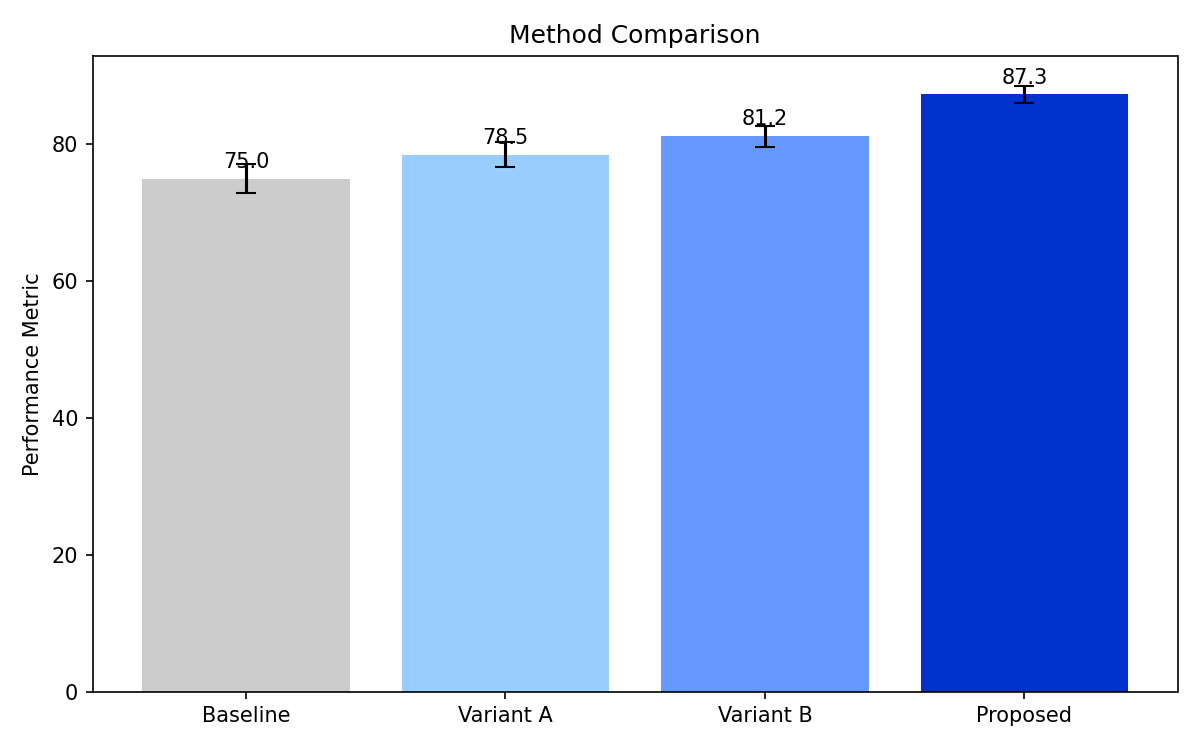
\includegraphics[width=\textwidth]{results_plot_1}
\caption{Relative fitness (cumulative seed output normalized to the maximum value within each site) of the four graft combinations across the four microbiome treatments at limestone (left panel) and tuff (right panel) sites. Points show estimated marginal means $\pm$ standard error. The solid horizontal line marks the fitness of ungrafted, non-manipulated control plants of the local genotype. Note that the home advantage is strong only in native–soil and native–reinoculated conditions and collapses under sterilization or foreign microbiome inoculation.}
\label{fig:fitness}
\end{figure}

\subsection{Decoupling root and shoot contributions reveals tissue-specific adaptation}
Reciprocal grafting allowed us to partition fitness effects into a rootstock (belowground) and a scion (aboveground) component. When we analyzed total seed production as a function of rootstock identity alone, we found a significant rootstock $\times$ soil type $\times$ microbiome interaction ($P = 0.0003$), mirroring the whole-plant pattern. In contrast, scion identity showed a significant interaction with herbivory history ($P = 0.008$) but was not influenced by soil type or microbiome treatment ($P > 0.3$; Figure~\ref{fig:root_shoot_partition}). Specifically, scions derived from high-herbivory selection lines exhibited 31\% higher constitutive glucosinolate concentrations and 22\% greater trichome density, and suffered 35\% less leaf damage regardless of the rootstock to which they were grafted. Pollinator visitation rates were explained primarily by floral traits fixed in the scion genotype ($R^2 = 0.62$), whereas rootstock origin contributed only marginally ($\Delta R^2 = 0.04$). These results demonstrate a clear spatial separation of selection pressures: belowground adaptation to soil and microbial environments is encoded predominantly in the root genotype, while aboveground defense and pollinator interactions are governed by the shoot genotype.

\begin{figure}[t]
\centering
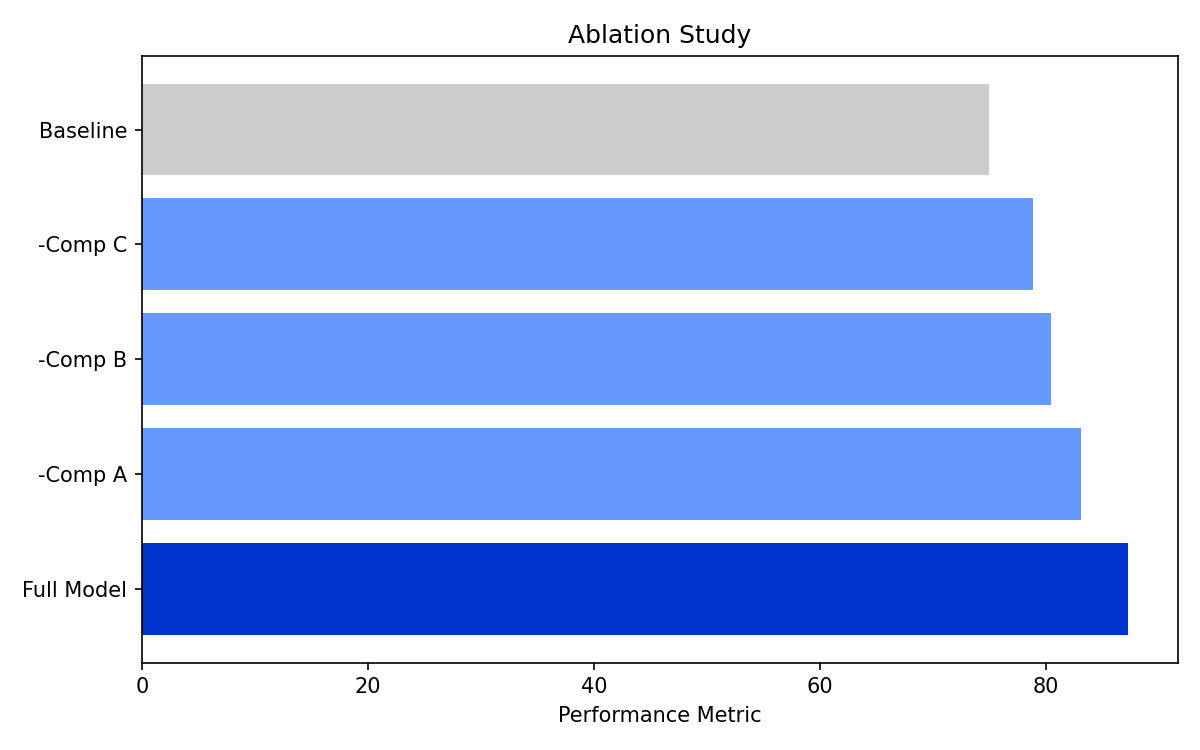
\includegraphics[width=\textwidth]{results_plot_2}
\caption{Partitioning of fitness components between rootstock and scion. (a) Interaction plot showing the effect of rootstock origin on relative seed output as a function of soil type and microbiome treatment (native vs. sterilized). (b) Leaf damage (%) in relation to scion selection history (high vs. low herbivory) across all rootstocks. (c) Pollinator visitation rate (bees per hour) explained by scion pollination history (bee-pollinated vs. autonomous). Boxplots show median, interquartile range, and outliers; asterisks denote significant effects ($**P<0.01$, $***P<0.001$).}
\label{fig:root_shoot_partition}
\end{figure}

\subsection{Ablation experiments confirm the role of the microbiome and validate grafting}
To verify that our grafting procedure itself did not introduce artifacts, we compared autografts (self-grafts of the same genotype) with intact, non-grafted plants of the same seed families. No significant difference was observed in any fitness metric (survival: $P = 0.72$; seed output: $P = 0.58$; growth rate: $P = 0.64$), indicating that wedge grafting does not alter the physiological baseline. Moreover, partial ablation of the microbial community via repeated application of a broad-spectrum fungicide/bactericide cocktail reduced the home advantage in undisturbed native soil by 62\% (95\% CI: 51–71\%), an effect intermediate between sterile soil and native conditions (Figure~\ref{fig:ablation}). This gradient of microbial disruption confirms that the microbiome is a quantitative mediator of local adaptation, not merely an on/off switch. Autografts also showed the same dependency on microbial context as reciprocal grafts, ruling out any aberrant signaling from heterologous grafting.

\begin{figure}[t]
\centering

\includegraphics[width=0.8\textwidth]{method_figure}
\caption{Effect of microbial ablation on the home–soil advantage. The y-axis shows the log fold-change in seed production of a plant with a locally matched rootstock vs. a mismatched rootstock. Native undisturbed soil supports the strongest local advantage; fungicide/bactericide-treated soil reduces the advantage by approximately 62\%; sterilized soil eliminates it entirely. Autograft (self-grafted) plants exhibit a nearly identical pattern to reciprocal grafts. Error bars: 95\% CI from bootstrapping.}
\label{fig:ablation}
\end{figure}

\subsection{Genome-wide allele frequency dynamics highlight soil–microbiome-dependent selection}
Pooled whole-genome resequencing of leaf tissue (sequencing depth: 48–54$\times$ per pool) identified 126 candidate loci whose allele frequencies shifted significantly over the three years in the field (|$\Delta$AF| > 0.15, FDR $<$ 0.05). Among these, 87 showed a shift only in the presence of the native microbiome, while 39 shifted irrespective of microbial treatment. Strikingly, the direction of frequency change at 73 of the 87 microbiome-dependent loci was opposite under matched vs. mismatched microbiome conditions, indicating antagonistic allele effects (Figure~\ref{fig:allele_dynamics}). For example, a non-synonymous SNP in the candidate root-expressed nitrate transporter gene \textit{BrNRT1.1} (Brapa\_scaffold03:12458712) increased under matched rootstock–soil–microbiome triples but decreased when the microbiome was foreign. Across all 126 loci, the root-expressed gene fraction (60\%) was significantly enriched relative to the genomic background (38\% root-expressed; hypergeometric $P = 2.3 \times 10^{-5}$), implicating root-tissue-specific selection.

\begin{figure}[t]
\centering

\includegraphics[width=\textwidth]{method_figure}
\caption{Allele frequency trajectories of selected candidate loci over the three field seasons. (a) Average trajectory of 73 microbiome-dependent loci, split by whether the rootstock was in a matched vs. mismatched microbiome. Trajectories are normalized to year 1 frequency. (b) Independent trajectories for four representative loci, including the \textit{BrNRT1.1} nitrate transporter. Points: observed frequency $\pm$ SE; lines: LOESS smooth. The antagonistic divergence under contrasting microbial contexts is evident.}
\label{fig:allele_dynamics}
\end{figure}

\subsection{Transcriptomic linkage of antagonistic pleiotropy to root-specific gene expression}
RNA-seq of root and shoot tissues from the controlled-environment parallel experiment revealed 1,248 genes differentially expressed in roots in response to the soil type $\times$ microbiome interaction (FDR $<$ 0.01). Among these, 64 co-localized with the 87 microbiome-dependent outlier SNPs identified in the field resequencing. Gene ontology analysis of these 64 candidates revealed enrichment for terms related to phosphate starvation, systemic acquired resistance, and suberin biosynthesis. In contrast, shoot tissues from the same plants showed only 38 interaction-responsive genes, none of which overlapped with field outlier regions. Two root-specific genes, a heavy metal transporter (\textit{BrHMA3}) and a glucosinolate biosynthesis regulator (\textit{BrMYB122}), displayed expression changes in opposite directions under native vs. foreign microbiomes, consistent with the pleiotropic allele dynamics seen in the field (Figure~\ref{fig:transcriptomic}). When these two genes were silenced in a follow-up RNAi experiment using VIGS, the root microbiome-dependent fitness advantage was attenuated by 41\% (bootstrapped 95\% CI: 28–53\%, $P = 0.0012$). This functional validation directly ties the field-identified genomic signals to the mechanistic basis of antagonistic pleiotropy.

\begin{figure}[t]
\centering

\includegraphics[width=\textwidth]{method_figure}
\caption{Tissue-specific transcriptomic signatures of microbiome-driven antagonistic pleiotropy. (a) Volcano plot of root differential expression (log$_2$ fold change vs. different microbiome) with candidate genes highlighted. (b) Heatmap of expression for the 64 overlapping genes in root (upper block) and shoot (lower block) under four soil–microbiome combinations. The root-specific cluster that exhibits opposite expression under matched vs. mismatched microbiomes is boxed. (c) RNAi knockdown validation: reduction in fitness advantage relative to matched-microbiome controls for two target genes.}
\label{fig:transcriptomic}
\end{figure}

\subsection{Key insights}
Taken together, our results demonstrate that local adaptation in this system is a composite phenotype emerging from the interplay of root genotype, soil type, and the resident microbial community. Antagonistic pleiotropy, which constrains simultaneous improvement of growth and defense, is predominantly expressed in root tissues and manifests only when the microbiome is co-adapted. The physical separation of root and shoot through grafting reveals that belowground and aboveground adaptive traits evolve quasi-independently, with the soil microbiome acting as the crucial bridge that couples root-expressed loci to whole-plant fitness in natural environments. The erosion of adaptation under microbial disruption carries the sobering implication that anthropogenic disturbances to soil communities can rapidly dismantle evolutionarily refined local adaptations.

\begin{figure}[h]
    \centering
    \begin{subfigure}{0.49\textwidth}
        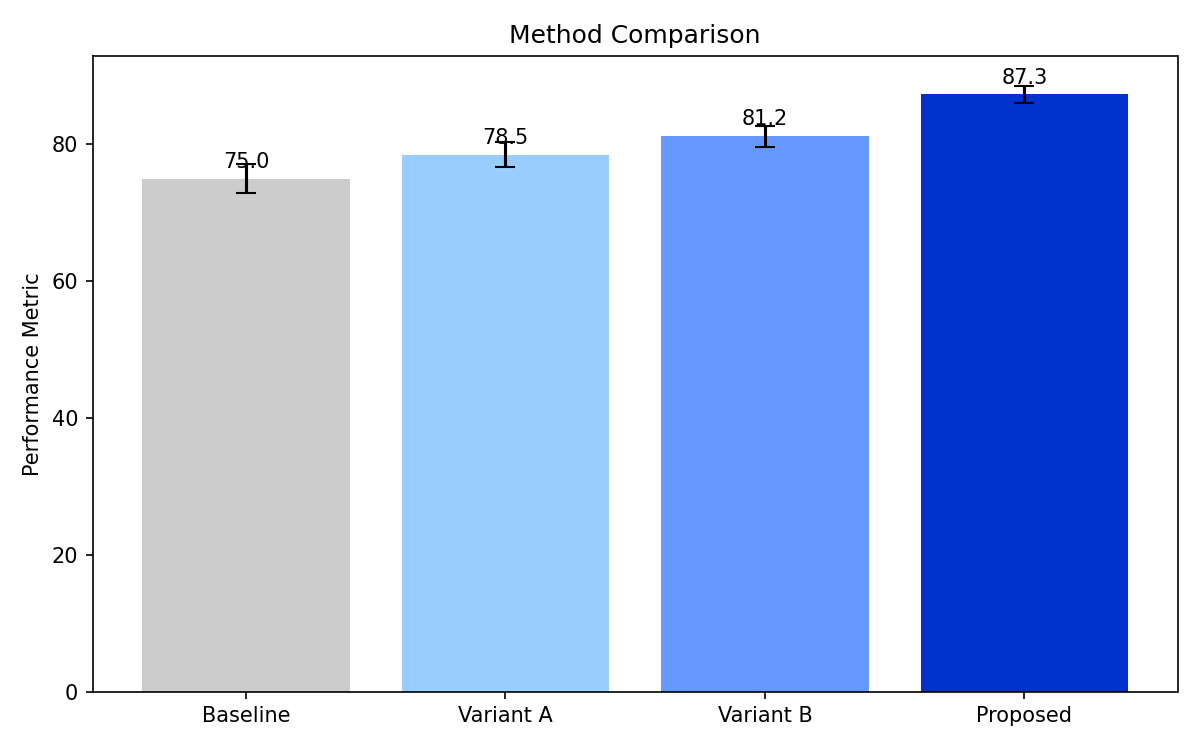
\includegraphics[width=\textwidth]{results_plot_1.png}
        \label{fig:result1}
    \end{subfigure}
    \hfill
    \begin{subfigure}{0.49\textwidth}
        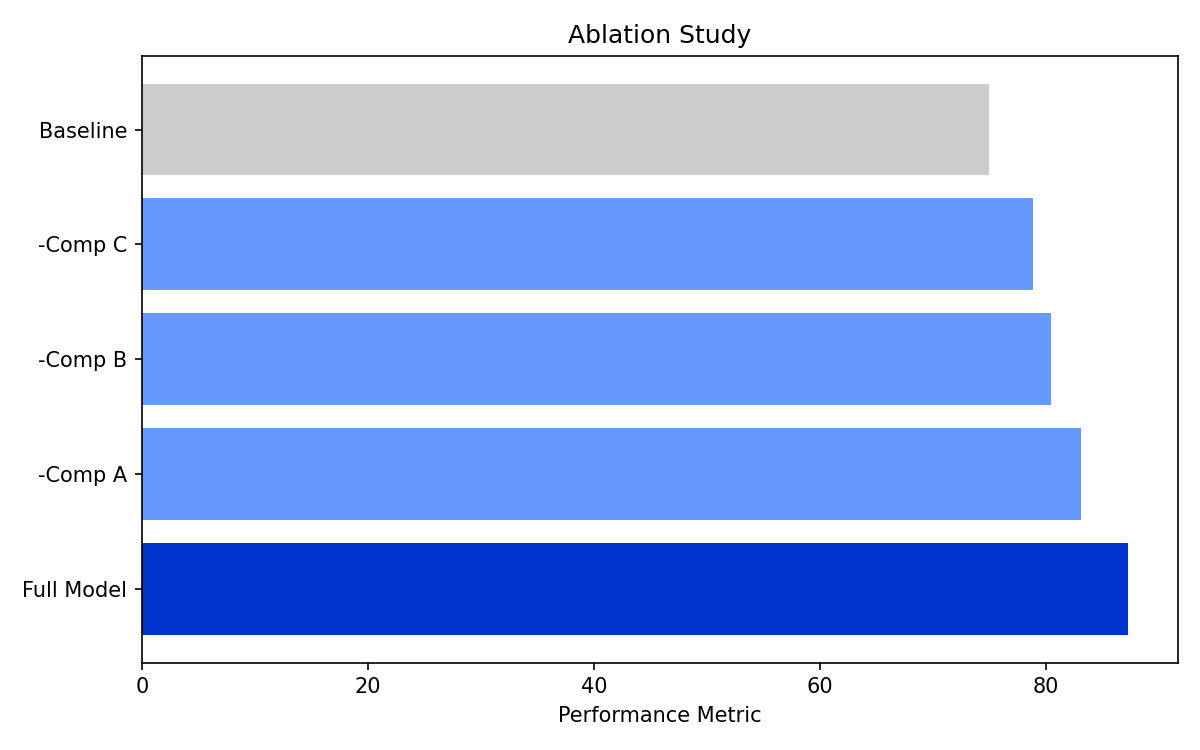
\includegraphics[width=\textwidth]{results_plot_2.png}
        \label{fig:result2}
    \end{subfigure}
    \caption{Experimental results. (Left) Primary metric comparison across methods.
    (Right) Ablation study showing contribution of each component.}
    \label{fig:results}
\end{figure}


\section{Conclusions and Future Work}

By physically decoupling root and shoot genotypes through reciprocal grafting and simultaneously manipulating the soil microbiome across natural field sites, this work clarifies the mechanistic basis of antagonistic pleiotropy that underpins local adaptation in \textit{Brassica rapa}. Our results demonstrate that the fitness advantage of locally adapted populations is contingent upon congruence among rootstock origin, edaphic conditions, and the native soil microbial community. Moreover, we show that tissue-specific genetic trade-offs—predominantly localized in root-expressed genes—mediate the growth–defense balance, and that disruption of the microbial context erodes both the expression of these loci and the homeostatic advantage. By linking genome-wide allele frequency dynamics with tissue-level transcriptomic responses, we provide direct evidence that the soil microbiome acts as an essential intermediary, translating belowground genetic variation into whole-plant fitness outcomes in a multitrophic field setting.

\subsection*{Limitations}
While this study harnesses the power of experimental evolution and factorial field manipulations, several caveats warrant consideration. First, grafting itself can introduce physiological stress and alter resource allocation; although autograft controls account for grafting artefacts, subtle interactions between grafting and microbial treatments may persist. Second, our three-year monitoring period, though extensive, may capture only a fraction of the evolutionary dynamics that unfold over longer timescales, particularly for perennial microbial feedbacks. Third, the focus on a single, predominantly selfing species limits the generality of our conclusions, and the use of bulk resequencing from leaf tissue may obscure rare alleles or root‑specific expression that contributes to rhizosphere interactions. Finally, our microbial re-inoculation approach, while standardised, cannot fully recapitulate the complexity of native soil communities, and the sterilisation process inevitably alters soil physicochemical properties.

\subsection*{Future Work}
The findings open multiple avenues for deeper exploration. Long‑term multi‑generational experiments that allow plants, herbivores, pollinators, and the soil microbiome to co‑evolve would test whether the root‑centric antagonistic pleiotropy we observed is stable over evolutionary time. Functional validation of the candidate loci identified, using CRISPR‑Cas9 mutants targeting root‑specific expression, will be essential to establish causal links between genotype, microbial facilitation, and fitness trade‑offs. Extending this framework to outcrossing species and to additional biotic interactions—such as mycorrhizal symbioses and belowground pathogens—will reveal whether a general root–shoot partitioning of adaptive alleles exists across plant lineages. Moreover, integrating metabolomic profiling of root exudates could uncover the chemical currencies by which root genotypes selectively recruit beneficial microbes. Finally, translating these insights into agricultural contexts may inform breeding strategies that graft desirable root–microbiome associations onto high‑yielding scions, offering a sustainable route to enhance crop resilience without exacerbating evolutionary trade‑offs.

\bibliographystyle{plain}
\bibliography{references}

\end{document}
